\begin{figure}[t!]
     \centering
        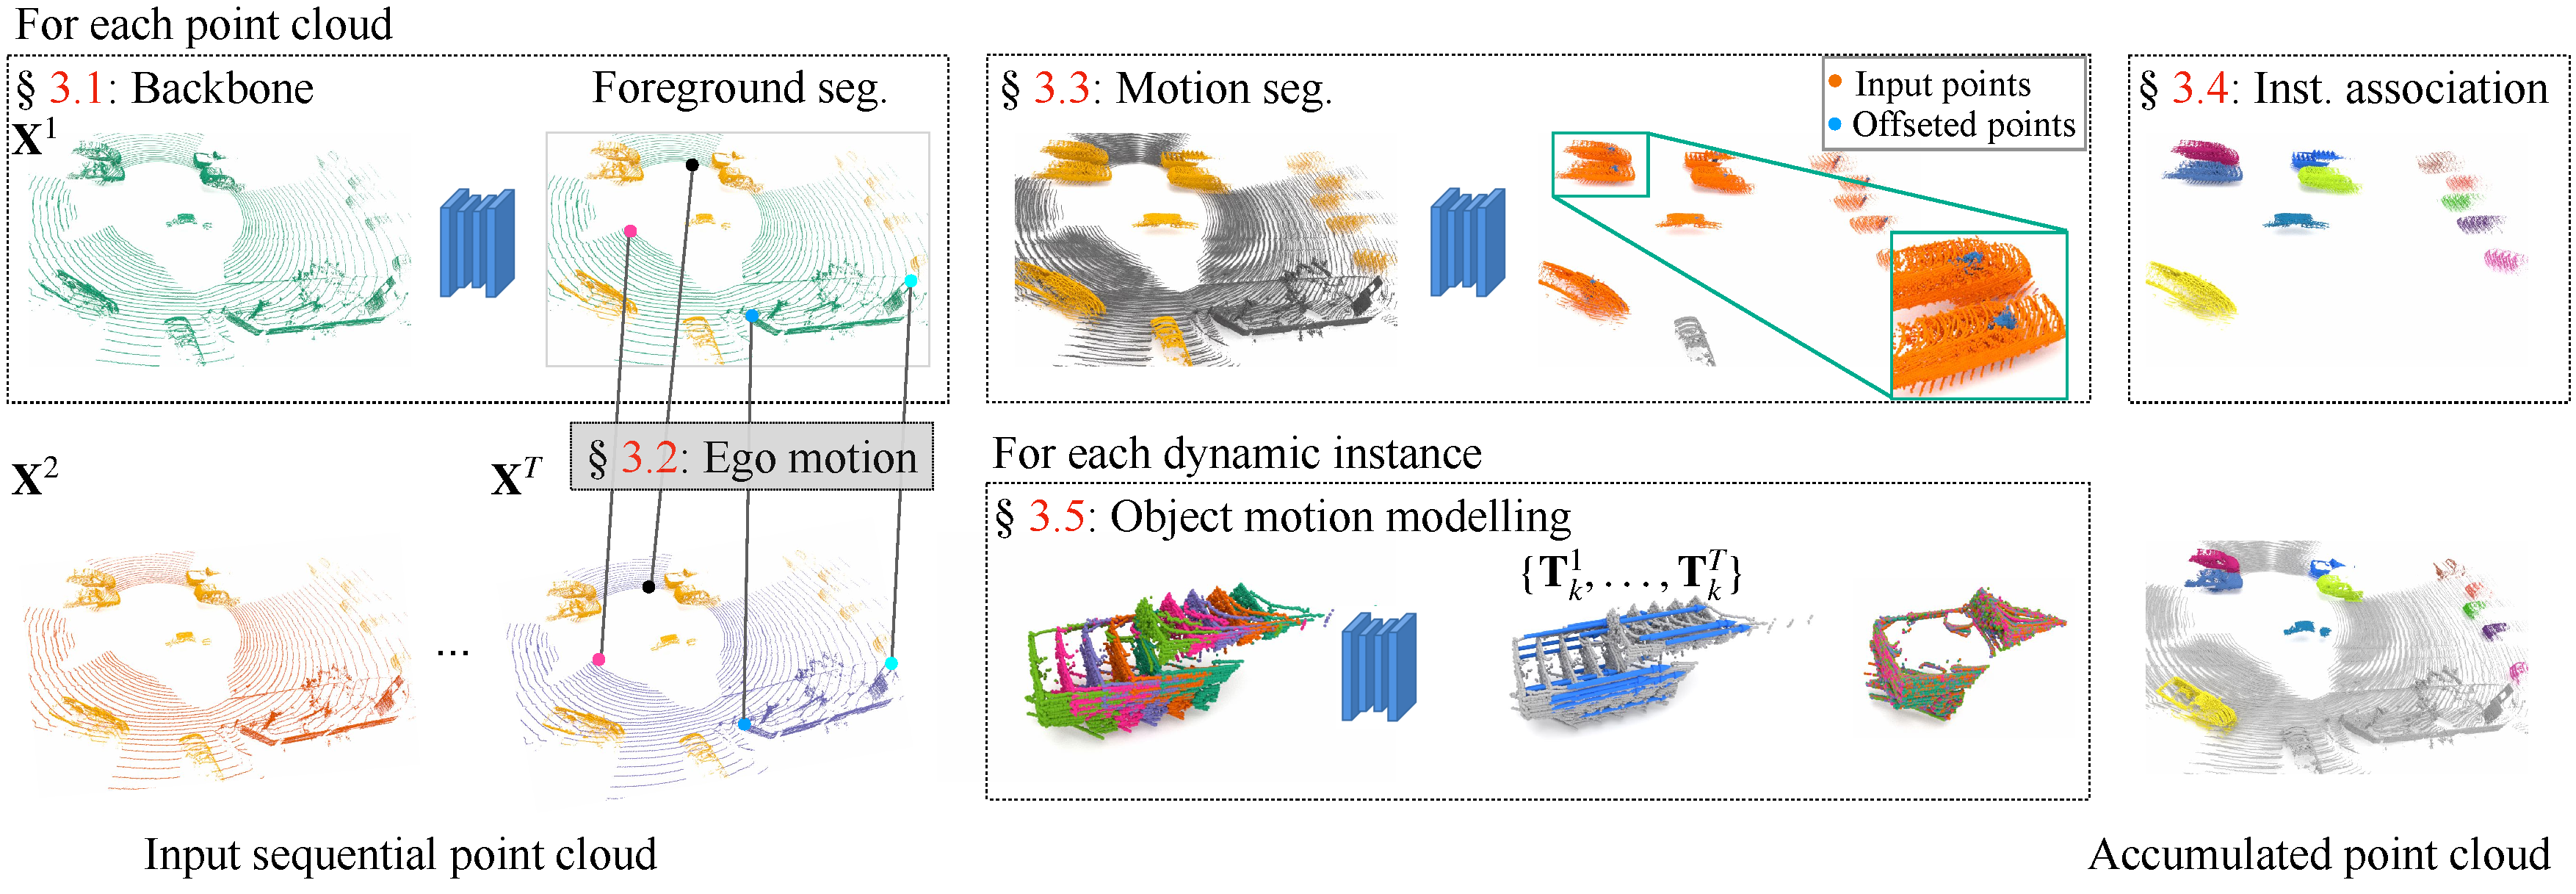
\includegraphics[width=1.0\columnwidth]{figs/figure/overview.pdf}
        \caption{\textbf{Overview}. Our method takes in a point cloud sequence of $T$ frames and starts by extracting foreground points (marked {\setlength{\fboxsep}{0pt}\colorbox{yellow}{yellow}}) for each frame. To obtain ego motion, $T-1$ pairwise registrations are performed. %
       Next, points belonging to dynamic foreground object are extracted using our motion segmentation module (marked {\setlength{\fboxsep}{0pt}\colorbox{tab10orange}{orange}}).
       To boost subsequent spatio-temporal instance association, we additionally predict per-point offset vectors. After instance association, we finally compute the rigid motion separately for each segmented dynamic object.}
        \label{fig:architecture}
\end{figure}